\subsection{Diagramma delle classi lato Server}
	\begin{figure}[H]
	\centering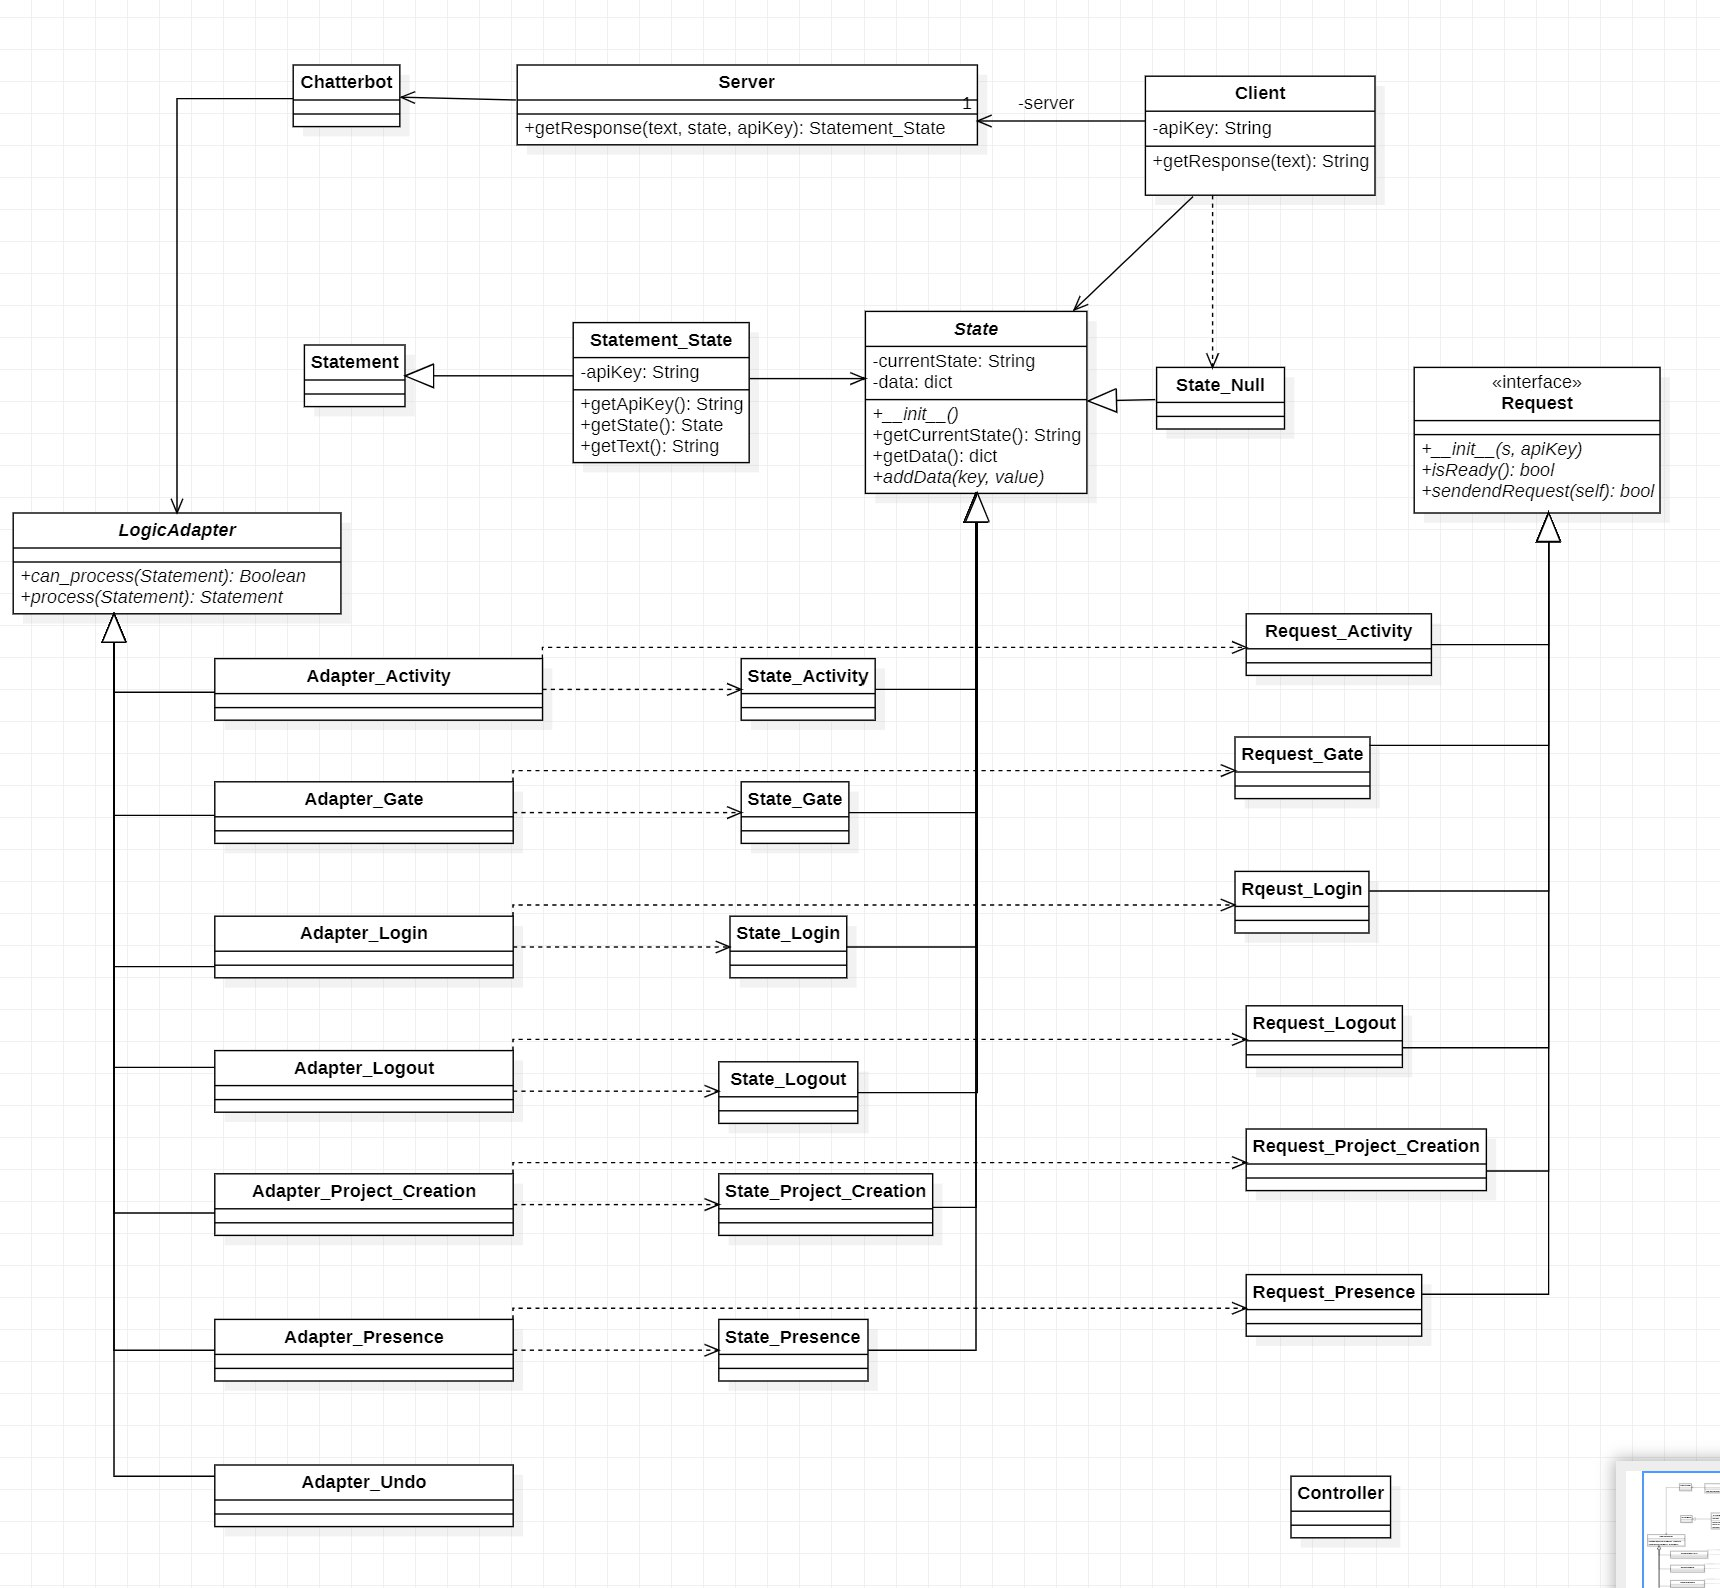
\includegraphics[scale=0.70]{images/diagramma_classi.jpg}
    \caption{Diagramma UML delle classi lato Server}
	\end{figure}

\newpage

\subsection{Server}
\subsubsection{App} Unico punto dell'applicativo dove viene interfacciato l'utente, qui viene istanziato il server e la lista dei client. Inoltre viene definito il routing delle richieste del client grazie al framework Flask. 
\subsubsection{Client} Classe che rappresenta ogni client connesso. Quando viene istanziata mantiene lo stato interno della richiesta, e con il metodo getResponse trasmette la richiesta al server.
\subsubsection{Server} Classe che inizializza la libreria esterna \textit{Chatterbot}. Presenta il metodo getResponse, il quale crea lo \textit{Statement\_State} con i parametri forniti dal Client e scorre tutti gli adapter cercando di rispondere in modo corretto alla richiesta. 
\subsubsection{Chatterbot} Classe della libreria esterna \glossario{Chatterbot}. Rappresenta un istanza del ChatBot e tutti gli adapter ad esso collegati.
\subsubsection{Statement} Classe della libreria esterna \glossario{Chatterbot}. Rapprensenta un input che il ChatBot riceve o un output che il ChatBot ritorna in merito all'input ricevuto.
\subsubsection{LogicAdapter} Classe della libreria esterna \glossario{Chatterbot}. Determina la logica di come il ChatterBot seleziona la risposta allo Statement di input. I suoi due metodi can\_process e process sono il fulcro dell'applicativo lato server. can\_process determina se una richiesta può essere soddisfatta dall'adapter, process definisce come elaborarla. Questa classe viene usata come classe base astratta per tutti gli adapter, questi infatti ereditano da LogicAdapter i due metodi e li sovvrascrivono per creare la propria logica di risposta.
\subsubsection{State} Interfaccia che definisce il contratto di tutti i vari stati. Presenta i tre metodi che gli stati implementano per assolvere ognuno alla propria funzione. All'interno di ogni State saranno definiti i dati, in forma di dizionario (chiave, valore),  necessari per completare la richiesta e su questi implementati i vari metodi. In generale getCurrentState ritornerà lo stato corrente, getData ritornerà i dati definiti all'interno di ogni State e addData aggiungerà un dato al dizionario.
\paragraph*{State\_Null} Implementa l'interfaccia \textit{State}, di particolare importanza perchè non è associato a nessun adapter. Serve per simulare lo stato nullo, viene utilizzato quando l'utente non è in nessun'altro stato.
\subsubsection{Statement\_State} Sottoclasse di Statement (classe della libreria esterna \glossario{Chatterbot}). Estende lo Statement di Chatterbot con lo State e l'ApiKey della richiesta. 
\subsubsection{Request} Interfaccia che definisce tutte le request. Presenta due metodi isReady e sendRequest il quale funzionamento verrà implementato per ogni request. In generale isReady verifica se la request è pronta per essere inviata, mentre invece sendRequest invia la richiesta \glossario{HTTP} alle \glossario{API Rest} di Imola Informatica per interagire con i loro servizi, e ritorna una risposta per verificare se la richiesta è andata a buon fine o meno.
\subsubsection{Login} Classi \textit{Adapter\_Login}, \textit{State\_Login} permettono di effettuare il login
\subsubsection{Logout} Classe \textit{Adapter\_Logout} permette di effettuare il logout.
\subsubsection{Activity} Classi \textit{Adapter\_Activity}, \textit{State\_Activity} e \textit{Request\_Activity}. 
per la funzionalità di consuntivare le ore dedicate ad un progetto compreso le eventuali ore di viaggio.
\subsubsection{Gate} Classi \textit{Adapter\_Gate}, \textit{State\_Gate} e \textit{Request\_Gate} per la funzionalità di apertura cancello
\subsubsection{Project\_Creation} Classi \textit{Adapter\_Project\_Creation}, \textit{State\_Project\_Creation} e \textit{Request\_Project\_Creation}
\subsubsection{Presence} Classi \textit{Adapter\_Presence}, \textit{State\_Presence} e \textit{Request\_Presence} per la funzionalità di registrazione della presenza
\subsubsection{Undo} Classe \textit{Adapter\_Undo} permette di annullare l'operazione in corso e di ricominciare la stessa o un'altra operazione dall'inizio.
\subsection{Diagramma di sequenza Esecuzione Richiesta}
\newpage

\begin{landscape}
	\begin{figure}[H]
	\centering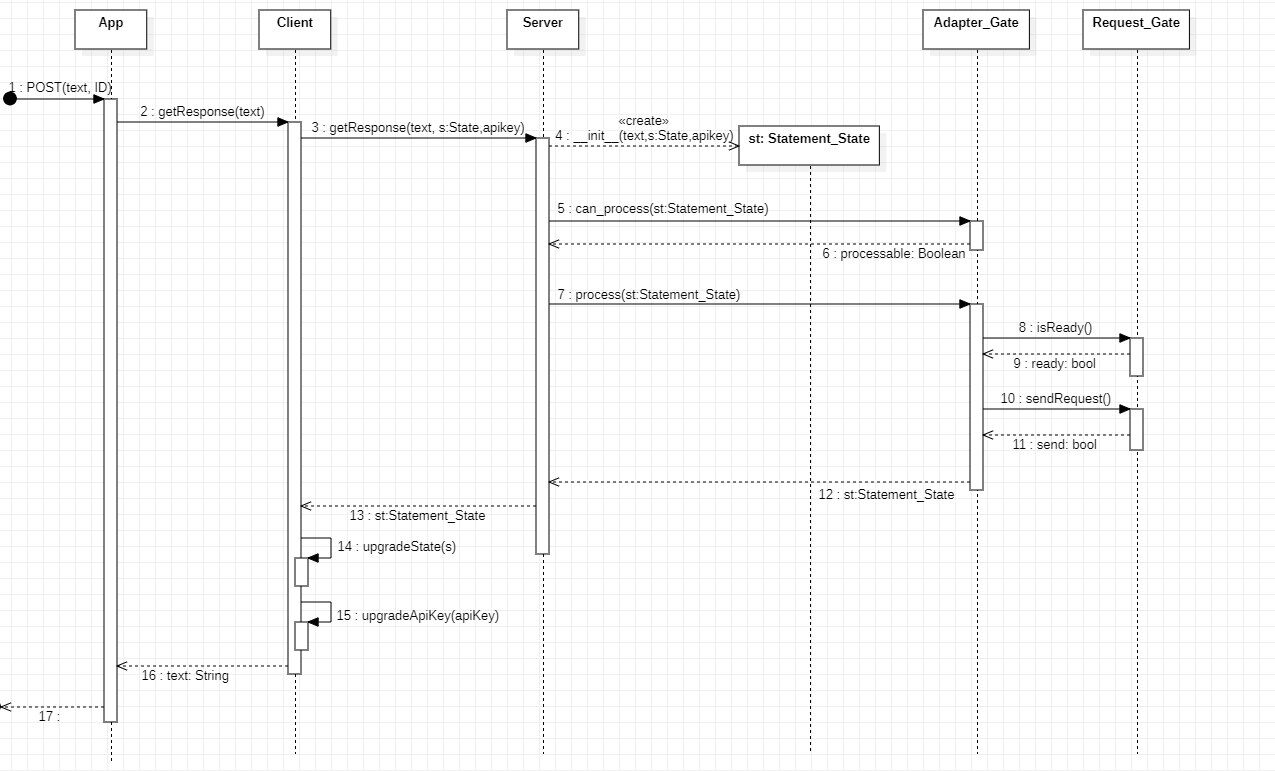
\includegraphics[width=\linewidth]{images/diagramma_sequenza_server.jpg}
    \caption{Diagramma di sequenza Esecuzione Richiesta }
	\end{figure}
\end{landscape}
\begin{itemize}
    \item Il \glossario{Client} web effettua una richiesta POST all'\textit{App}, che si compone di testo inserito dall'utente (text) e identificativo univoco del \textit{Client} connesso (ID).
    \item \textit{App} riceve la richiesta, seleziona il corretto \textit{Client} che deve gestirla mediante l'ID ricevuto e inoltra a \textit{Client} il testo della richiesta invocando il metodo \textit{getResponse}.
    \item Il \textit{Client} richiama il metodo del \textit{Server} \textit{getResponse} passandogli il testo della richiesta, lo stato attuale della richiesta e l'\textit{ApiKey} con la quale la richiesta è stata effettuata.
    \item Il \textit{Server} riceve la richiesta del \textit{Client}, crea lo \textit{Statement\_State} con i tre dati che ha ricevuto, e invoca la libreria Chatterbot per cercare la risposta più pertinente al testo della richiesta (in questo caso "apertura cancello"). In questo caso il Server fa la richiesta ad \textit{Adapter\_Gate} con il metodo \textit{can\_process}, passando come paramentro lo \textit{Statement\_State} che ha creato.
    \item \textit{Adapter\_Gate} risponde con un boolean alla richiesta per determinare se può processarla o meno, e lo ritorna al \textit{Server}.
    \item Il server richiama \textit{Adapter\_Gate} per processare la richiesta passando come parametro lo \textit{Statement\_State} che ha creato.
    \item \textit{Adapter\_Gate} prepara la richiesta, in base ai dati che ha ricevuto e verifica con il metodo \textit{isReady} di \textit{Request\_Gate} se questa è pronta per essere effettuata. \textit{Request\_Gate} risponde con un boolean indicando se la richiesta è pronta o meno per essere eseguita.
    \item Se la richiesta è pronta per essere effettuata (come nell'esempio) \textit{Adapter\_Gate} invoca il metodo \textit{sendRequest} di \textit{Request\_Gate} per effettuare realmente la richiesta verso le API di Imola Informatica. \textit{Request\_Gate} riponde con un boolean che indica se la richiesta è andata a buon fine.
    \item A questo punto \textit{Adapter\_Gate} ritorna lo \textit{Statement\_State} al server che aveva iniziato la richiesta con il metodo \textit{process}.
    \item Il \textit{Server} dopo aver ricevuto lo \textit{Statement\_State} in risposta dell'adapter lo trasmette al \textit{Client} che aveva fatto la richiesta \textit{getResponse}.
    \item Il \textit{Client} riceve lo \textit{Statement\_State}, aggiorna il proprio stato con il metodo \textit{upgradeState} e la propria \textit{ApiKey} con il metodo \textit{upgradeApiKey}. Infine ritorna ad \textit{App} la risposta sotto forma di string (text) perchè venga indirizzata al \glossario{Client} web.
\end{itemize}
\subsection{Diagramma di sequenza Richiesta Identificativo}
\begin{figure}[H]
    \centering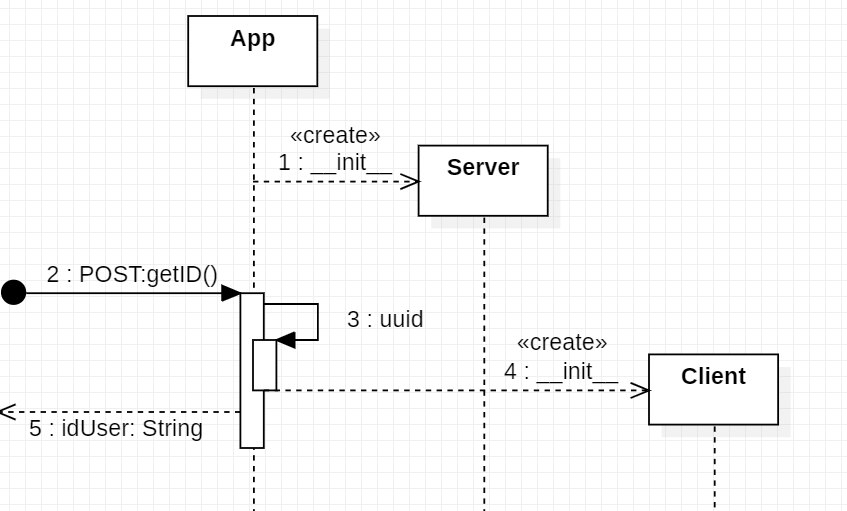
\includegraphics[width=\linewidth]{images/diagramma_sequenza_client.jpg}
    \caption{Diagramma di sequenza Richiesta Identificativo}
\end{figure}
\begin{itemize}
    \item Il \glossario{Client} web effettua una richiesta POST \textit{getID} ad \textit{App} richiedendo un ID.
    \item \textit{App} riceve la richiesta del nuovo Client che vuole connettersi al \textit{Server}, precedentemente creato e inizializzato, e crea un \glossario{UUID}, per identificarlo univocamente in tutte le comunicazioni.
    \item \textit{App} in seguito crea ed inizializza un \textit{Client} nuovo associato al ID appena creato.
    \item Infine \textit{App} ritorna al \glossario{Client} web l'identificativo univoco creato sotto forma di un campo stringa (idUser).
\end{itemize}
\newpage